%\documentclass{article}
\documentclass[conference]{IEEEtran}

%package list for graphics and text functions
\usepackage[utf8]{inputenc}
\usepackage{graphicx}
\graphicspath{ {./images/} }
\usepackage[export]{adjustbox}
\usepackage{subcaption}
\usepackage{wrapfig}

\usepackage{cite}
\usepackage{amsmath,amssymb,amsfonts}
\usepackage{algorithmic}
\usepackage{textcomp}
\usepackage{xcolor}
\def\BibTeX{{\rm B\kern-.05em{\sc i\kern-.025em b}\kern-.08em
    T\kern-.1667em\lower.7ex\hbox{E}\kern-.125emX}}


\title{Differentiation of Renal Clear Cell Carcinoma and Oncocytoma Using Deep Learning Methods}


\author{\IEEEauthorblockN{Erdi Kidane}
\IEEEauthorblockA{\textit{UCLA} \\
Los Angeles, USA \\
Erdi.Kidane@engineering.ucla.edu}
\and
\IEEEauthorblockN{Xuesen Cui}
\IEEEauthorblockA{\textit{UCLA} \\
Los Angeles, USA \\
cuixuesen@ucla.edu}
\and
\IEEEauthorblockN{Keane Gonzalez}
\IEEEauthorblockA{\textit{} 
Los Angeles, USA \\
kgonza@g.ucla.edu}
}

\date{June 2019}

\begin{document}



\maketitle

\section{Introduction}
More than 47,000 Americans have died from some form of kidney disease, this number is higher than deaths due to breast and prostate cancer [1]. Of this group, 13,570 deaths are due specifically to kidney cancer\cite{b2}.  The most common renal malignancy is called renal cell carcinoma (RCC), which alone, accounts for 3\% of all types of cancers within the United States\cite{b3} . According to the National Institutes of Health indicates that the real rate of new kidney cancer diagnosis not due to improvement in detection methods is also increasing\cite{b3}.  

Medical history is often considered when screening for RCC.  Beyond this there is no other standardized screening test for this disease\cite{b4}.  The current most commonly used method to detect lesions within the kidneys are CT scans.  Once a mass in detected further, more invasive and expensive analysis is required to determine whether it is benign or malignant.  As a rule, masses without microscopic fat are to be considered malignant\cite{b5} until proven otherwise via further testing. 

By imaging with and without contrast and during differing phases of the contrast life within the renal tissue, it was possible to more clearly differentiate various areas of the kidney mass as the contrast is washed out of the organ. Being able to selectively mark and filter out non-lesion boundaries based upon the tissue shown from various phases allowed them to more clearly contour regions of interest. 

Recent work attempts to differentiate between benign and malignant masses via Google’s TensorFlow software with the goal of automating and generalizing the method of characterization enough to be widely applicable and subjecting patients to less invasive procedures. As the data set includes annotation margins provided by trained radiologists, it's known which images have or do not have target lesions in them. This labeling could be utilized to train a classification model to possibly automatically detect whether an image shows signs of RCC or an oncocytoma.

\section{Materials and Methods}

\subsection{Data Preparation}

The original data set, from the a selection of patient cases at UCLA\cite{b5}, comprised 118 patients with annotated renal clear cell carcinoma indications and 36 patients diagnosed with oncocytoma indications. Annotated file sets, which contained the margins for the lesion or tumors noted by a radiologist, written in MetaFile format produced with the ITK toolset\cite{b9}, were provided for each renal phase of every patient.

For every patient, four phases of data taken during unique phases of kidney filtration. The pre-contrast phase was taken without the use of a contrasting agent. After taking this baseline image, a contrast solution was injected into each patient, a timing setup was used to image during specific filtering stages of the kidney: corticomedullary, nephrographic, and excretory. The contrast levels were at different stages of processing during each timing step, which provided slightly altered images for each stage.

The raw DICOM images for each phase were processed using the PyDicom\cite{b8} python library to read in the DICOM tags and raw pixel data. The annotation data, as part of an ITK file, provided the volume of the tumor marked for each patient\footnote{The data only includes margins for a single tumor, whether clear cell carcinoma or an oncocytoma}. This dataset had a single tumor annotated for the study, but this does not mean there were not other tumors present. For the purposes of this project, we use the single annotation as a truth set for our labeling needs.

Dealing with large amounts of data, almost 40GB in this case, required settling on a data organization scheme. For this data set, it was decided that keeping the original delineations of clear cell and oncocytoma would be the simplest. For each type of dataset, the clear cell and oncocytoma directories, there existed a folder for each patient\footnote{Patient names were replaced with date/time and generic IDs during a previous use of the data}. Underneath each patient folder there were subfolders containing CT information for the pre-contrast and three target phases of renal filtration (corticomedullary, nephrographic, and excretory).

The model requires data with clear cell carcinoma and oncocytoma, but our input data consisted of the raw DICOM pixel data. Each DICOM file contained one slice of the patient, which included areas of no interest to our needs, such as CT bed, non-kidney parenchyma, and empty air. Including these extra entities might negatively bias our model, so a more localized set of the raw data was needed. 

To obtain an image set that included data central to our needs, the radiologist annotation data was used to select only those axial plane slices that were deemed to have a target tumor. This not only limited the number of images that would go into training, but ensured that only data with features of interest were being used.\\

%
% Include the raw image/subset/lesion plot 
%
\begin{figure}[h]
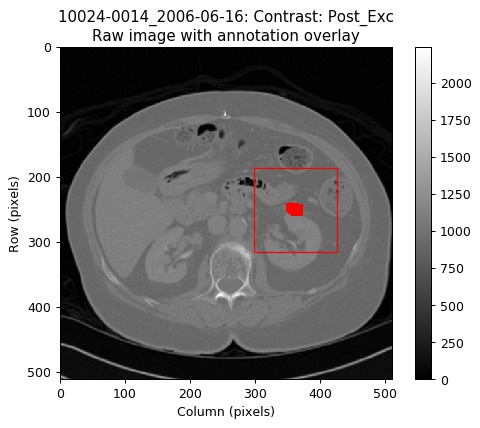
\includegraphics[width=9cm]{annotation_10024-0014_2006-06-16_0045}
\caption{Raw DICOM slice with the subset image bounding box and overlay of radiologist lesion margins}
\label{fig:RawSubLesion}
\end{figure}

For each patient image of every renal phase, a small subset was taken of each valid slice (red outline in Figure \ref{fig:RawSubLesion}). This was centered around the middle pixel of the annotated lesion (the slice containing the middle of the lesion in the axial slices) denoted by the solid red area in Figure  \ref{fig:RawSubLesion}. \\
The boundary box for the final setup was chosen to be 128 pixels in width and height. This parameter was decided to be large enough to contain the largest lesion margins with some padding for extra tissue, but small enough to not encompass too many other organs. \\ %get to a new line
By including not only features/textures from the lesion areas, but from normal renal tissue too, this should have provided further information on lesion tissue attached to normal tissue.

One line of thinking was that the model may benefit from having lesion textures/features combined with normal tissue. A downside to this, is that patient physiology differed widely and the center of a lesion could be within the center of a kidney or on the outer edge of the organ. Lesions on the outer edges, combined with placement of the kidneys for some patients had the possibility of including unwanted tissue areas into the subset image.\\
The example shown in Figure \ref{fig:subim1} details how the sample subimage, \ref{fig:subim2}, includes the entirety of the lesion in that slice, but also includes some unwanted tissue. A majority of the cases included lesion volumes well within the kidney volume, which meant that training data would be ideal and which should offset some of the less ideal cases, as shown in Figures \ref{fig:raw with subset} and \ref{fig:Slice through center of lesion margin}, where \ref{fig:Slice through center of lesion margin} shows a data slice through the center of the lesion image in \ref{fig:subim1}. Depending on the test image, a simple delineation between the tissue of concern and surrounding tissue may not be as clear.

\hfill \\
%Include a paired image set with raw and subset shown
\begin{figure}[hb!]
    \begin{subfigure}{0.65\textwidth}
    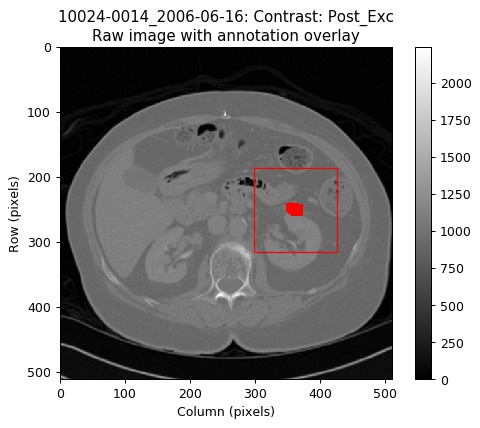
\includegraphics[width=0.8\linewidth, height=6cm]{annotation_10024-0014_2006-06-16_0045} 
    \caption{Raw With subset}
    \label{fig:subim1}
    \end{subfigure}
    \begin{subfigure}{0.65\textwidth}
    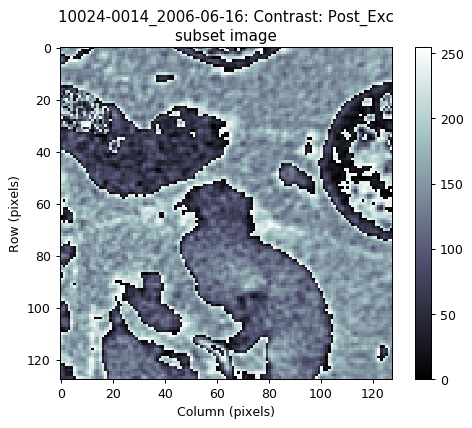
\includegraphics[width=0.8\linewidth, height=6cm]{subset_10024-0014_2006-06-16_0045}
    \caption{Subset of raw image}
    \label{fig:subim2}
    \end{subfigure}
    \caption{Raw dicom and chosen subset}
    \label{fig:raw with subset}
\end{figure}

\hfill \\
\newpage


\begin{figure}[h]
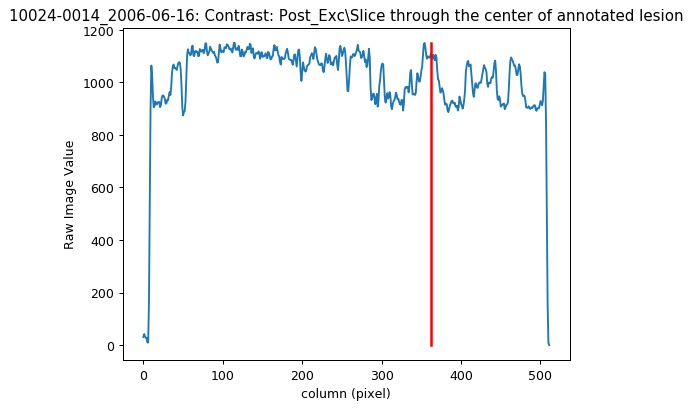
\includegraphics[width=9cm]{data_slice_10024-0014_2006-06-16_0045}
  \caption{Data slice through center of lesion in median slice of lesion}
  \label{fig:Slice through center of lesion margin}
\end{figure}


\hfill \\

\subsection{Model Input Data}
For use in our model setup, the DICOM pixel data was trimmed down to a 128 x 128 pixels 2D image size and saved as a generic JPEG formatted image file. Each specific test (one for each of four phases and all four phases per patient) produced a varying number of images, depending on the volume of the lesion margins noted by the reviewers (in essence, one JPEG image was generated for each slice that contained any part of the lesion volume, centered around the middle of the lesion). Since the lesions were not uniform throughout the patients, this resulted in differing numbers of input images depending on the patient. \\

\subsection{Methods}
A pre-trained model, Inception\footnote{version 3 of Inception provided the most functionality for our needs}\cite{b10}, was utilized as a starting point for adding features from our dataset. This version was previously trained to an accuracy of 78.7\%\footnote{Using the ILSVRC 2012 validation data, it succesfully predicted 39371/50000 example labels}. Our test images were trained alongside this model to detect RCC or oncocytoma.\\
Essentially, Inception, is a deep learning tool that uses a convolutional neural network (CNN) which is a network designed specifically for imaging data.  It works by having different layers where each layer transforms a 3D volume input to a 3d volume output using some differentiable function that could have parameters. \\ 
For example, a layer in our deep learning model has learned to focus on edges in a certain region of the kidney. The following layer may focus on the overall kidney to pick out some other feature.  In order to accomplish this the layer in question needs an appropriate filter size to detect something different.\\  
At this point what the inception layer allows internal layers to do is pick and choose different filter sizes and determine the one that is most relevant to learn the required information.  Thus, even if there is a variance in image sizes the layer will work to recognize desired features.

%Inception architecture
\begin{figure}[h]
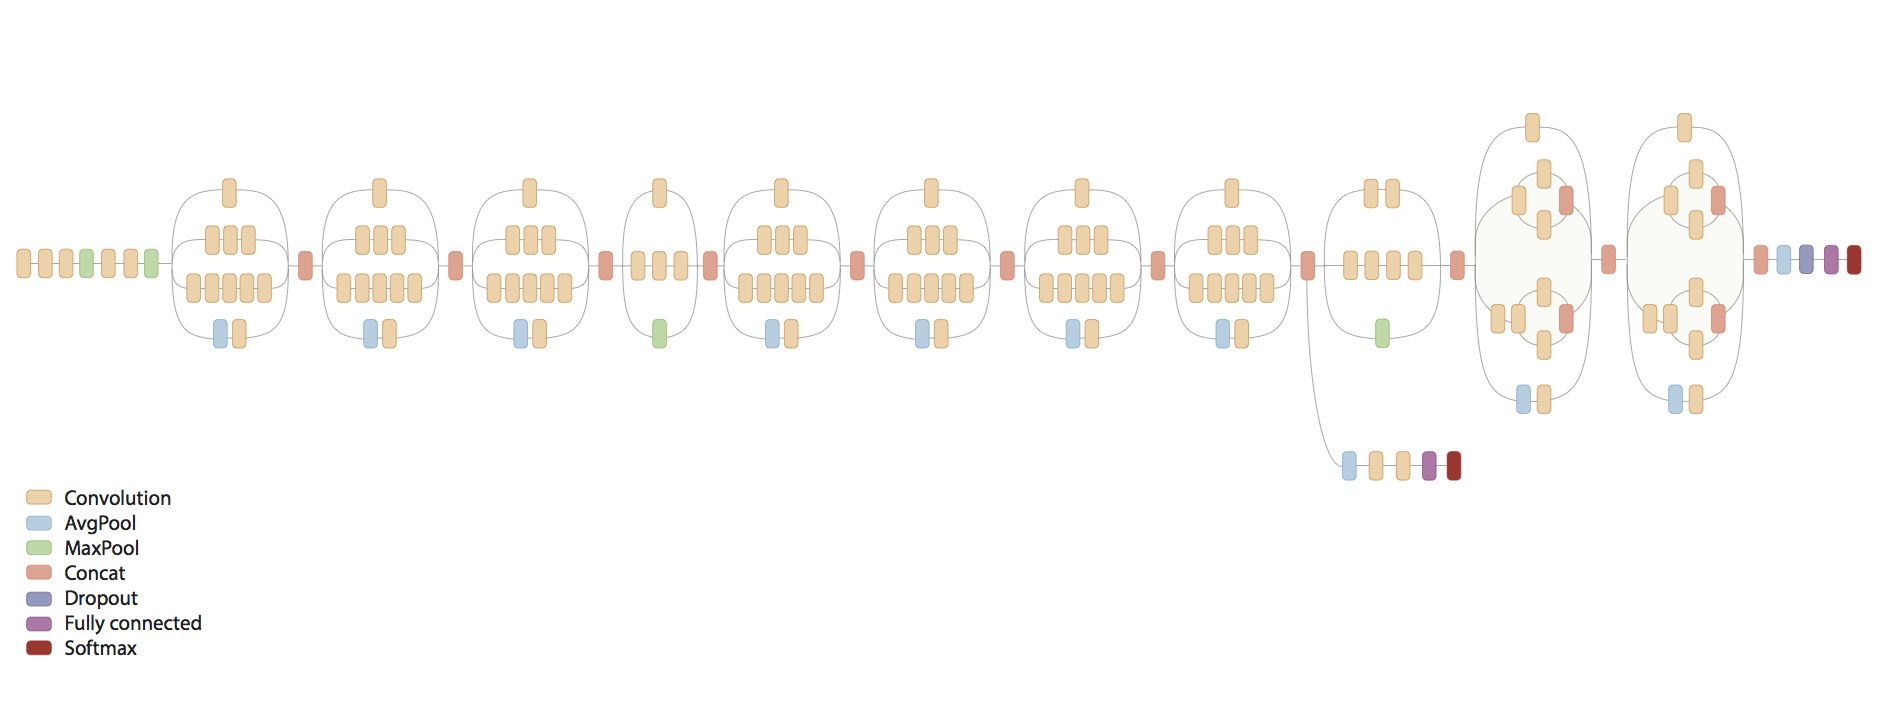
\includegraphics[width=9cm]{inception_v3_architecture.png}
  \caption{Architecture of Inception V3 Model}
  \label{fig:Inception Model}
\end{figure}


The input images added were taken from the combined set of data to include the RCC set and the oncocytoma set. Of these, 500 images were dedicated for training, with 250 images used for testing. Approximately \(\frac{2}{3} \) of the of the images for training were taken from each patient and the remaining \(\frac{1}{3} \) used for testing.
\hfill \\




\subsection{Results}

The model was trained with varying numbers of input images, with the final accuracy leveling off at approximately 90\% as shown in Figure \ref{fig:Model Accuracy}. The number of images used for training and validation was altered to get the best results, with 90\% providing the best results for the amount of computation time needed.

%Accuracy plot
\begin{figure}[h]
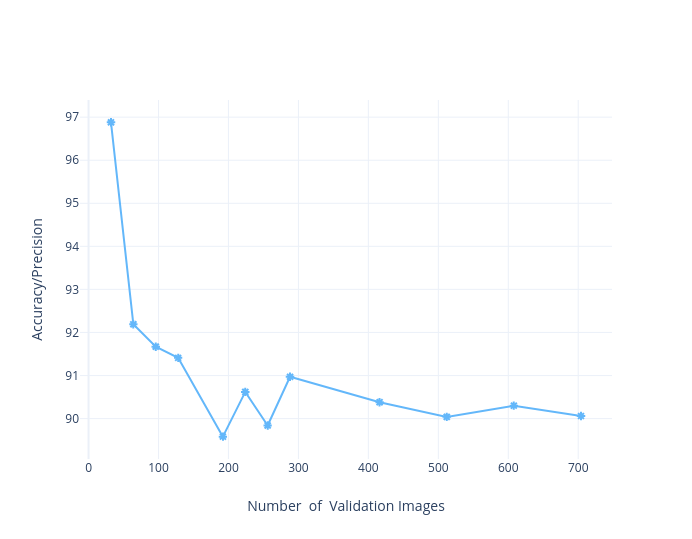
\includegraphics[width=9cm]{Accuracy_Plot.png}
  \caption{Model Accuracy as number of images increased}
  \label{fig:Model Accuracy}
\end{figure}


\newpage

\subsection{Conclusion}

The model was able to achieve accurate classification 90\% of the time.  This is with a set of 700 training images and 250 images for testing.  We believe that given more training data we could’ve pushed this number higher as more images means more convolution layers producing a more accurate model.\\
Further, the model we picked was inception v3 however there is a more refined version called inception v4.  It introduces a specialized “Reduction Block” at different layers.  These blocks change the width and height of the grid and help speed up the computation when preforming convolution.  

One issue that may have had negatively biased our results was the process used for selecting subset patches. As the data was patient based, it was expected that not every patient would have identical organ placement and size (normal human variation), but the combination of patient uniqueness, where the target lesion margins were noted, and the fixed size of our input to the model allowed for non-kidney tissue to be captured, as seen in Figure \ref{fig:Spinal Intrusion}. Here, part of the spinal mass was incorporated into our model data.\\

\begin{figure}[h]
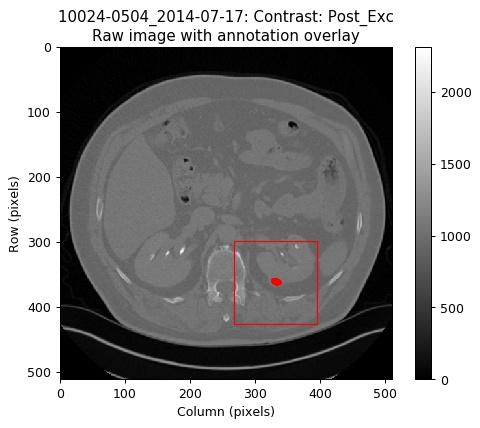
\includegraphics[width=9cm]{annotation_10024-0504_2014-07-17_0056}
  \caption{Raw DICOM with subset showing spinal intrusion}
  \label{fig:Spinal Intrusion}
\end{figure}

How much this affected our results (either negatively or in a false positive sense) needs to be investigated. There are many ways to avoid this, but the simplest change would be to use a smaller output image size (32 x 32 may have provided kidney only  textures/features at the expense of more area to process). The effect of changing the patch size used is another area of investigation that may yield better results. 

The target truth used, the annotation margins, also displayed some irregularities (possibly a normal part of the margin selection procedure), such as only existing in one slice or several cases not having valid annotations. Further review of why the annotations may have differed is needed, but for our use, those cases were not allowed to pass through for use in the model. 

\hfill \\
\listoffigures


%
% References Section
%
\begin{thebibliography}{00}
\bibitem{b1} C. G. Wood, L. J. Stromberg, C. B. Harmath, J. M. Horowitz, C. Feng, N. A. Hammond, D. D. Casalino, L. A. Goodhartz, F. H. Miller, and P. Nikolaidis, “CT and MR Imaging for Evaluation of Cystic Renal Lesions and Diseases,” RadioGraphics, vol. 35, no. 1, pp. 125–141, 2015. 
\bibitem{b2} W.-H. Chow, L. M. Dong, and S. S. Devesa, “Epidemiology and risk factors for kidney cancer,” Nature reviews. Urology, May-2010. [Online]. Available: https://www.ncbi.nlm.nih.gov/pmc/articles/PMC3012455/. [Accessed: 28-Apr-2019]. 
\bibitem{b3} Global Burden of Disease Cancer Collaboration. JAMA Oncol 2015; 1: 505-527 
\bibitem{b4} KB. Rini, S. C. Campbell, B. Escudeir, “Renal Cell Carcinoma,” The Lancet, vol 373, no 9669 Mar 2009 
\bibitem{b5} H. Coy, K. Hsieh, W. Wu, M. B. Nagarajan, J. R. Young, M. L. Douek, M. S. Brown, F. Scalzo, and S. S. Raman, “Deep learning and radiomics: the utility of Google TensorFlow™ Inception in classifying clear cell renal cell carcinoma and oncocytoma on multiphasic CT,” Abdominal Radiology, 2019. 
\bibitem{b6} “Kidney Cancer,” NHS Choices. [Online]. Available: https://www.nhs.uk/conditions/kidney-cancer/. [Accessed: 28-Apr-2019]. 
\bibitem{b7} R. S. Cotran, V. Kumar, T. Collins, and S. L. Robbins, Robbins pathologic basis of disease. Philadelphia: Saunders, 2007. 
\bibitem{b8} "PyDicom Library," [Online]. Available:https://github.com/pydicom/pydicom/. [Accessed: 5 June 2019].
\bibitem{b9} "ITK Toolkit,"  [Online]. Available: https://itk.org/. [Accessed: 5 June 2019]
\bibitem{b10} Christian Szegedy, Vincent Vanhoucke, Sergey Ioffe, Jonathon Shlens, Zbigniew Wojna, "Rethinking the Inception Architecture for Computer Vision," 2016 IEEE Conference on Computer Vision and Pattern Recognition, 2016
\end{thebibliography}







\end{document}
